%%%%%%%%%%%%%%%%%%%%%%%%%%%%%%%%%%%%%%%%%%%%%%%%%%%%%%%%%%%%%%%%%%%%%%%%

\begin{slide}{}
\normalsize

\begin{center}
Beispiel: Arithmetische Ausdr\"ucke
\end{center}
\vspace*{0.5cm}

\footnotesize
Beschreibung arithmetischer Ausdr\"ucke m\"oglich durch \\[0.3cm]
\hspace*{1.3cm} $G_{\mathtt{arith}} := \langle T, N, R, \textsl{Expr} \rangle$
\begin{enumerate}
\item $T = \{ \mathbf{number}, \mathbf{variable}, ``\mathtt{+}\symbol{34},
  ``\mathtt{-}\cq, ``\mathtt{*}\cq, ``\mathtt{/}\cq, ``\mathtt{(}\cq, ``\mathtt{)}\cq \}$
\item $N = \{ \textsl{Expr} \}$
\item Die Menge $R$ enth\"alt folgende Regeln 

      $\begin{array}{lcl}
      \textsl{Expr} & \rightarrow & \textsl{Expr}\; ``\mathtt{+}\cq \;\textsl{Expr} \\
                     & |           & \textsl{Expr}\; ``\mathtt{-}\cq \;\textsl{Expr}\\
                     & |           & \textsl{Expr}\; ``\mathtt{*}\cq \;\textsl{Expr}\\
                     & |           & \textsl{Expr}\; ``\mathtt{/}\cq \;\textsl{Expr}\\
                     & |           & ``\mathtt{(}\cq \;\textsl{Expr}\; ``\mathtt{)}\cq\\
                     & |           & \mathbf{number}\\
                     & |           & \mathbf{variable}\\
      \end{array}$
\end{enumerate}
Es gibt zwei Arten von Terminalen
\begin{enumerate}
\item \emph{W\"ortliche Terminale} stehen f\"ur sich selbst.

      Beispiel: $``\texttt{+}\cq,\; ``\texttt{-}\cq,\; ``\texttt{*}\cq,\; ``\texttt{-}\cq,\; ``\mathtt{(}\cq,\; ``\mathtt{)}\cq$

      Werden in Regeln durch\  ``\ und\ \cq\ abgegrenzt.
\item \emph{Token--Terminale} beschreiben Klassen von Strings und 
      werden durch regul\"are Ausdr\"ucke implementiert 

      \textbf{Beispiel}: $\mathbf{number}$, $\mathbf{variable}$
    
      werden in Beispielen $\mathbf{fett}$ gesetzt, klein geschrieben
\end{enumerate}
Nicht--Terminale werden \textsl{schr\"ag} gesetzt, gro\3 geschrieben

\textbf{Beispiel}: \textsl{Expr}

\vspace*{\fill}
\tiny \addtocounter{mypage}{1}
\rule{17cm}{1mm}
Kontext--freie Grammatik  \hspace*{\fill} Seite \arabic{mypage}
\end{slide}

%%%%%%%%%%%%%%%%%%%%%%%%%%%%%%%%%%%%%%%%%%%%%%%%%%%%%%%%%%%%%%%%%%%%%%%%

\begin{slide}{}
\normalsize

\begin{center}
Sprache einer Grammatik
\end{center}
\vspace*{0.5cm}

\footnotesize
\textbf{Gegeben}: Grammatik $G = \langle T, N, R, S \rangle$ mit $V = T \cup N$.

\textbf{Definition}: Falls
\begin{enumerate}
\item $X \in N$,
\item $\alpha, \beta, \gamma \in V^*$,
\item $(X \rightarrow \beta) \in R$
\end{enumerate}
ist, so sagen wir, dass \\[0.3cm]
\hspace*{1.3cm} $\alpha X \gamma \rightarrow \alpha \beta \gamma$ \\[0.3cm]
ein \emph{Ableitungs--Schritt}  ist.

Die \emph{transitive H\"ulle} von $\rightarrow$ bezeichen wir mit $\rightarrow^*$: \\
F\"ur $\alpha, \beta, \gamma \in V^*$ gilt also:
\begin{enumerate}
\item $\alpha \rightarrow^* \alpha$
\item Falls $\alpha \rightarrow \beta$ und $\beta \rightarrow^* \gamma$, so folgt $\alpha \rightarrow^* \gamma$
\end{enumerate}
\textbf{Sprechweise}: Falls $\alpha \rightarrow^* \gamma$ ist, sagen wir \\[0.3cm]
\hspace*{1.3cm}  $\alpha$ \emph{wird zu} $\gamma$ \emph{reduziert}

\textbf{Beispiel}: \\[0.3cm]
\hspace*{1.3cm} 
$
\begin{array}{lcl}
\textsl{Expr} & \;\rightarrow\; & \textsl{Expr}   \; ``\mathtt{+}\cq \;\textsl{Expr} \\
              & \;\rightarrow\; & \mathbf{number} \; ``\mathtt{+}\cq \;\textsl{Expr} \\
              & \;\rightarrow\; & \mathbf{number} \; ``\mathtt{+}\cq \;\mathbf{number}
\end{array}
$

\textbf{Definition}: Die Sprache $\Ll(G)$ ist \\[0.3cm]
\hspace*{1.3cm} $\Ll(G) := \{ \alpha \in T^* \;|\; S \rightarrow^* \alpha \}$

\vspace*{\fill}
\tiny \addtocounter{mypage}{1}
\rule{17cm}{1mm}
Kontext--freie Grammatik  \hspace*{\fill} Seite \arabic{mypage}
\end{slide}

%%%%%%%%%%%%%%%%%%%%%%%%%%%%%%%%%%%%%%%%%%%%%%%%%%%%%%%%%%%%%%%%%%%%%%%%

\begin{slide}{}
\normalsize

\begin{center}
Parse--B\"aume
\end{center}
\vspace*{0.5cm}

\footnotesize
Ein Wort aus $\Ll(G_{\mathtt{arith}})$ kann auf mehrere Weisen abgeleitet werden:
\begin{enumerate}
\item ``Richtige'' Ableitung \\[0.3cm]
\hspace*{1.3cm} 
$\begin{array}{lcl}
\textsl{Expr} & \;\rightarrow\; & \textsl{Expr}\; ``\mathtt{+}\cq\; \textsl{Expr} \\
              & \;\rightarrow\; & \mathbf{number}\; ``\mathtt{+}\cq\; \textsl{Expr} \\
              & \;\rightarrow\; & \mathbf{number}\; ``\mathtt{+}\cq\; \textsl{Expr}\; ``\mathtt{*}\cq\; \textsl{Expr} \\
              & \;\rightarrow\; & \mathbf{number}\; ``\mathtt{+}\cq\; \mathbf{number}\; ``\mathtt{*}\cq\; \textsl{Expr} \\
              & \;\rightarrow\; & \mathbf{number}\; ``\mathtt{+}\cq\; \mathbf{number}\; ``\mathtt{*}\cq\; \mathbf{number} \\
\end{array}
$
\vspace*{0.5cm}

Zugeh\"origer Parse--Baum: \\[0.8cm]
\hspace*{1.3cm} 
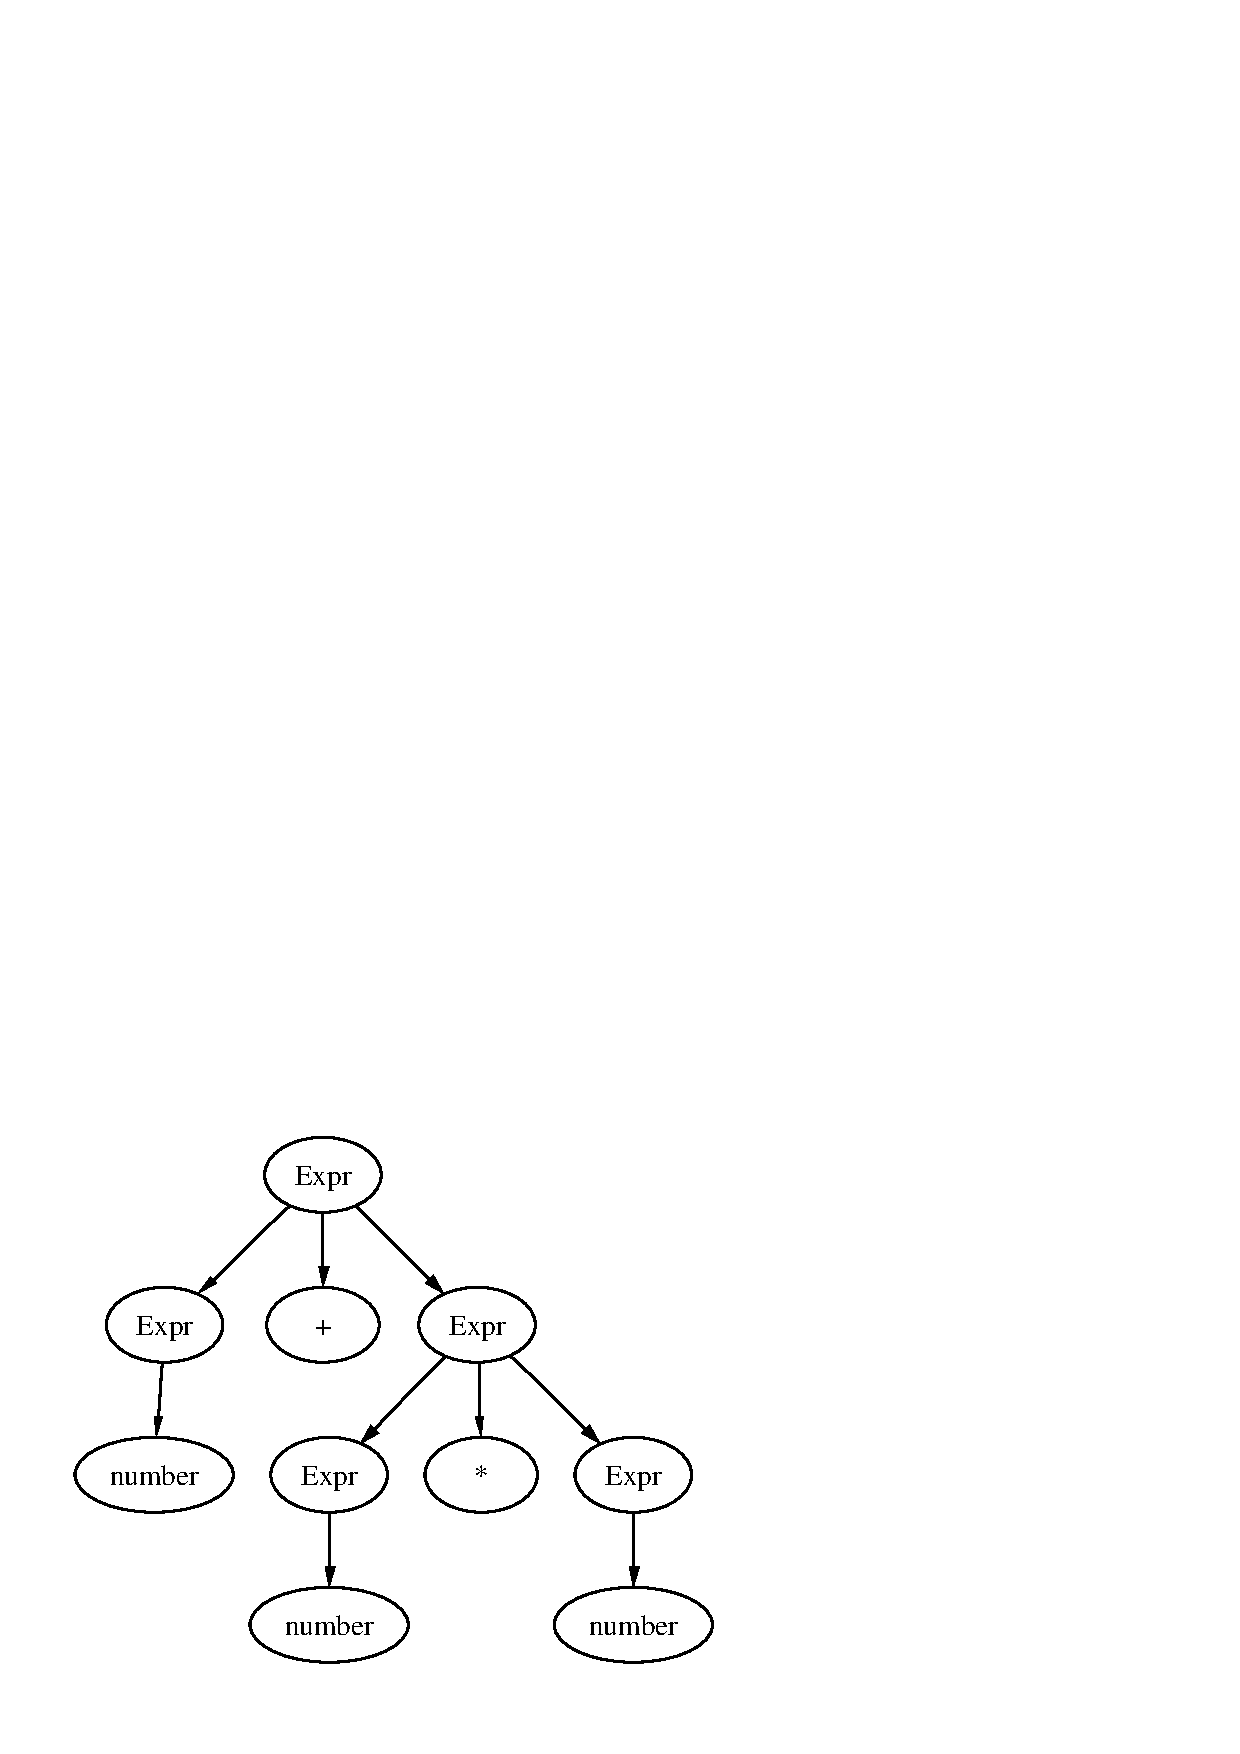
\epsfig{file=parse-tree1}

Entspricht dem Abarbeiten eines arithmetischen Ausdrucks der Form \\[0.3cm]
\hspace*{1.3cm} $x + y * z$
\end{enumerate}


\vspace*{\fill}
\tiny \addtocounter{mypage}{1}
\rule{17cm}{1mm}
Kontext--freie Grammatik  \hspace*{\fill} Seite \arabic{mypage}
\end{slide}

%%%%%%%%%%%%%%%%%%%%%%%%%%%%%%%%%%%%%%%%%%%%%%%%%%%%%%%%%%%%%%%%%%%%%%%%

\begin{slide}{}
\normalsize

\begin{center}
Parse--B\"aume (Fortsetzung)
\end{center}
\vspace*{0.5cm}

\footnotesize
\begin{enumerate}
\item ``Falsche'' Ableitung \\[0.3cm]
\hspace*{1.3cm} 
$\begin{array}{lcl}
\textsl{Expr} & \;\rightarrow\; & \textsl{Expr}\; ``\mathtt{*}\cq\; \textsl{Expr} \\
              & \;\rightarrow\; & \textsl{Expr}\; ``\mathtt{+}\cq\; \textsl{Expr}\; ``\mathtt{*}\cq\; \textsl{Expr} \\
              & \;\rightarrow\; & \textsl{number}\; ``\mathtt{+}\cq\; \textsl{Expr}\; ``\mathtt{*}\cq\; \textsl{Expr} \\
              & \;\rightarrow\; & \textsl{number}\; ``\mathtt{+}\cq\; \textsl{number}\; ``\mathtt{*}\cq\; \textsl{Expr} \\
              & \;\rightarrow\; & \textsl{number}\; ``\mathtt{+}\cq\; \textsl{number}\; ``\mathtt{*}\cq\; \textsl{number} \\
\end{array}
$
\vspace*{0.5cm}

Zugeh\"origer Parse--Baum: \\[0.8cm]
\hspace*{1.3cm} 
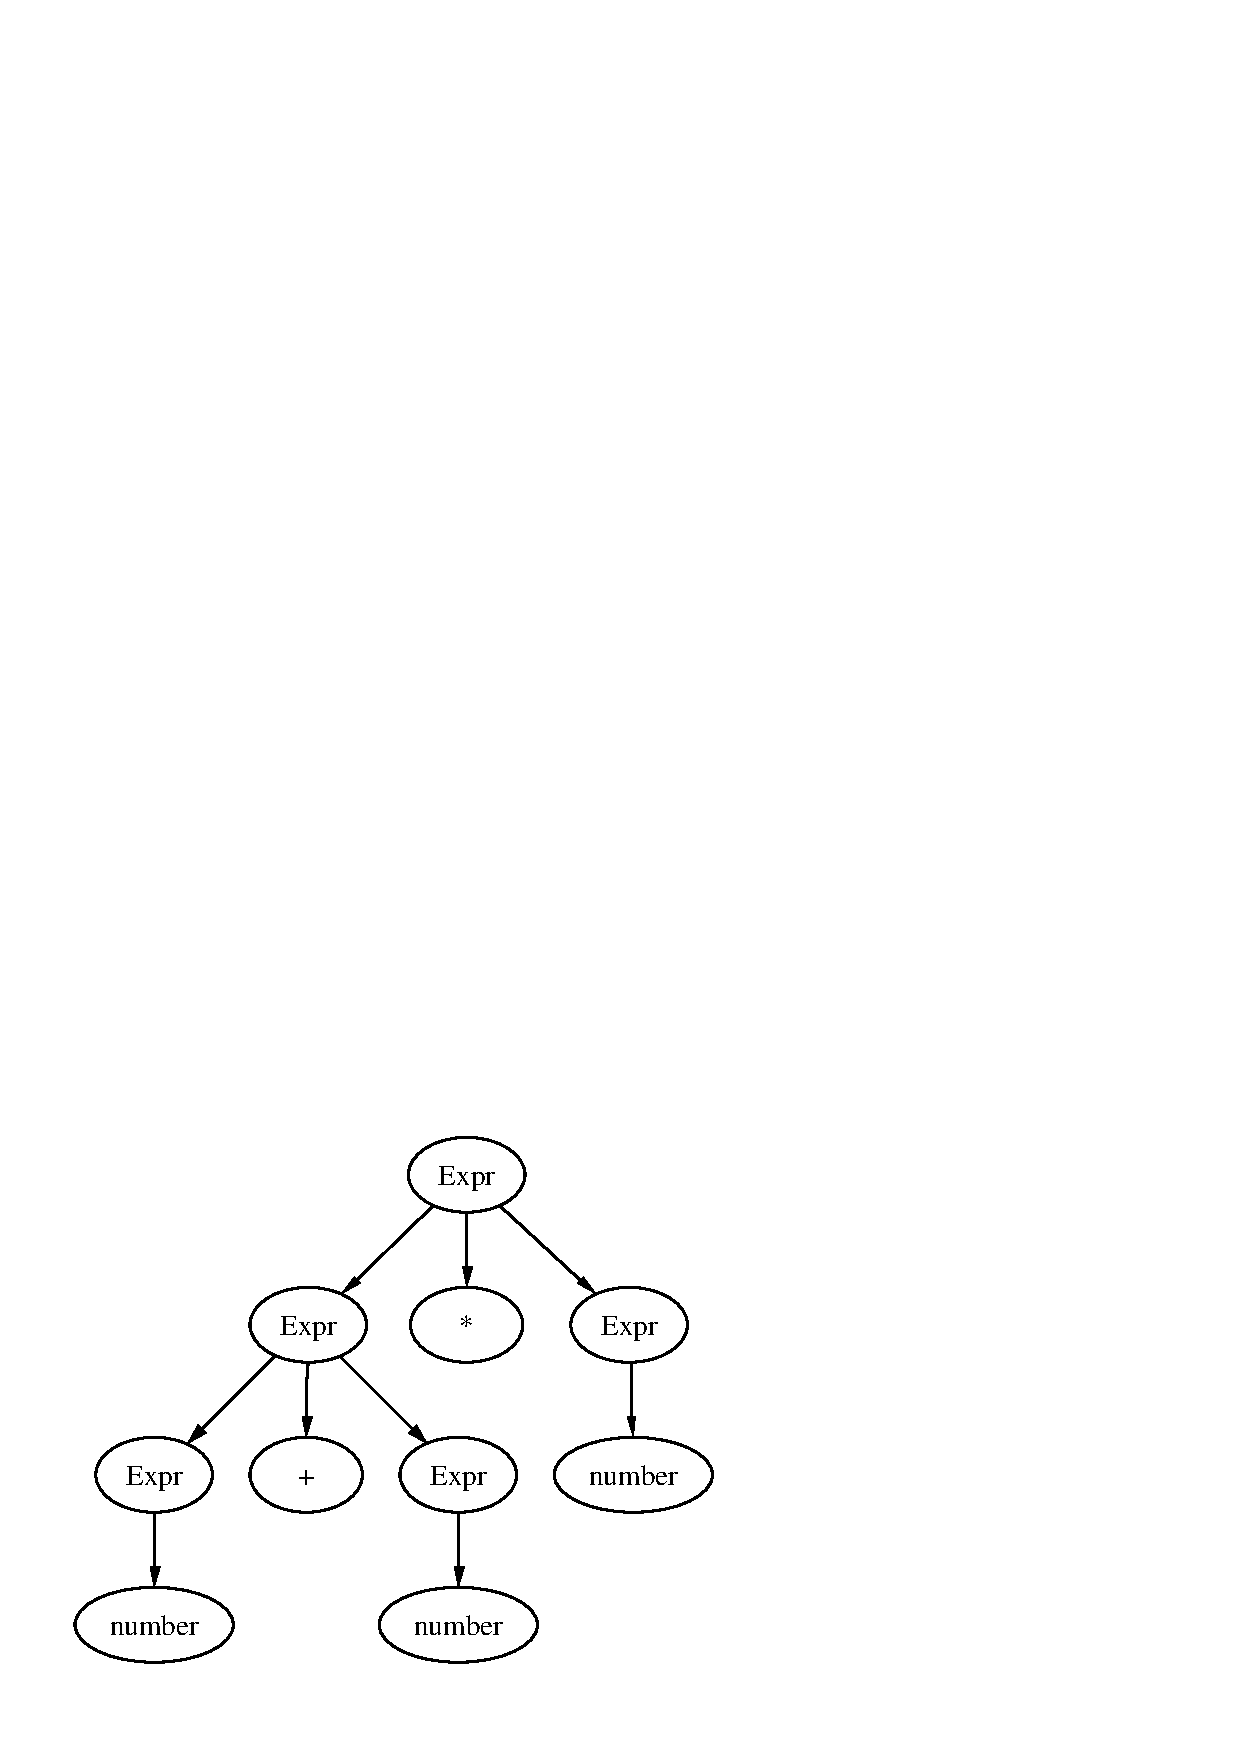
\epsfig{file=parse-tree2}

Abgeleitet wurde $x + y * z$

Parse--Baum entspricht aber \\[0.3cm]
\hspace*{1.3cm} $(x + y) * z$
\end{enumerate}

\textbf{Problem}: Grammatik $G_{\mathtt{arith}}$ ist \emph{mehrdeutig}!

\vspace*{\fill}
\tiny \addtocounter{mypage}{1}
\rule{17cm}{1mm}
Kontext--freie Grammatik  \hspace*{\fill} Seite \arabic{mypage}
\end{slide}

%%%%%%%%%%%%%%%%%%%%%%%%%%%%%%%%%%%%%%%%%%%%%%%%%%%%%%%%%%%%%%%%%%%%%%%%

\begin{slide}{}
\normalsize

\begin{center}
Grammatik f\"ur regul\"are Ausdr\"ucke
\end{center}
\vspace*{0.5cm}

\footnotesize
Beschreibung regul\"arer Ausdr\"ucke m\"oglich durch \\[0.3cm]
\hspace*{1.3cm} $G_{\mathtt{RegExp}} = \langle T, N, R, \textsl{Expr} \rangle$
\begin{enumerate}
\item $T = \{ \mathbf{letter}, \mathbf{escape}, ``\mathtt{+}\symbol{34},  ``\mathtt{*}\cq, ``\mathtt{(}\cq, ``\mathtt{)}\cq\}$
\item $N = \{ \textsl{Expr}, \textsl{Term}, \textsl{Factor} \}$
\item Die Menge $R$ enth\"alt folgende Regeln 

      $\begin{array}{lcl}
       \textsl{Expr} & \rightarrow & \textsl{Term}\; ``\mathtt{+}\cq \textsl{Expr} \\
                     & |           & \textsl{Term}                                 \\[0.3cm]
       \textsl{Term} & \rightarrow & \textsl{Factor}\;\textsl{Term}                  \\
                     & |           & \textsl{Factor}                                 \\[0.3cm]
       \textsl{Factor} & \rightarrow & ``\mathtt{(}\cq \;\textsl{Expr}\; ``\mathtt{)}\cq \; ``\mathtt{*}\cq\\
                     & |           & ``\mathtt{(}\cq \;\textsl{Expr}\; ``\mathtt{)}\cq\\
                     & |           & \mathbf{letter}\; ``\mathtt{*}\cq\\
                     & |           & \mathbf{letter}\\
                     & |           & \mathbf{escape}\; ``\mathtt{*}\cq\\
                     & |           & \mathbf{escape}\\
     \end{array}$
\end{enumerate}
Grammatik  eindeutig! Wurde erreicht durch \emph{Priorit\"aten}: \\[0.3cm]
\hspace*{1.3cm}  $\textsl{Factor}\; > \;\textsl{Term}\; > \;\textsl{Expr}$

entspricht Priorit\"at der Operations--Symbole
\begin{enumerate}
\item Abschluss ``\texttt{*}\cq
\item Konkatenation
\item Alternative ``\texttt{+}\cq
\end{enumerate}

\vspace*{\fill}
\tiny \addtocounter{mypage}{1}
\rule{17cm}{1mm}
Kontext--freie Grammatik  \hspace*{\fill} Seite \arabic{mypage}
\end{slide}

%%%%%%%%%%%%%%%%%%%%%%%%%%%%%%%%%%%%%%%%%%%%%%%%%%%%%%%%%%%%%%%%%%%%%%%%

\begin{slide}{}
\normalsize

\begin{center}
Beispiele f\"ur $\Ll(G_{\mathtt{RegExp}})$
\end{center}
\vspace*{0.5cm}

\footnotesize
Interpretation der Terminale

Sei $\Sigma$ Menge aller \sc{Ascii}--Zeichen. 
\begin{enumerate}
\item $\mathbf{letter}$: Alle Zeichen au\3er $``\mathtt{+}\cq,\; ``\mathtt{*}\cq,\; ``\mathtt{(}\cq,\;
``\mathtt{)}\cq,\; ``\mathtt{\symbol{92}}\cq$, also \\[0.3cm]
      \hspace*{1.3cm} $\Ll(\mathbf{letter}) = \Sigma \,\backslash\, \{ ``\mathtt{+}\cq,\; ``\mathtt{*}\cq,\; ``\mathtt{(}\cq,\;
``\mathtt{)}\cq,\; ``\mathtt{\symbol{92}}\cq \}$
\item $\mathbf{escape}$: W\"orter, die aus zwei Zeichen bestehen, wobei das erste Zeichen
      ein Backslash ``$\symbol{92}$'' ist: \\[0.3cm]
      \hspace*{1.3cm} $\Ll(escape) = \{ c_1c_2 \in \Sigma^* \;|\; c_1 = ``\mathtt{\symbol{92}}\cq \}$

      Semantik:
      \begin{enumerate}
      \item $\mathtt{\symbol{92}e}$ steht f\"ur $\varepsilon$
      \item $\mathtt{\symbol{92}}c$ mit $c \not= \mathtt{e}$ steht f\"ur $c$

            notwendig, um mit regul\"aren Ausdr\"ucken nach \\[0.3cm]
            \hspace*{1.3cm} $``\mathtt{+}\cq,\; ``\mathtt{*}\cq,\; ``\mathtt{(}\cq,\; ``\mathtt{)}\cq,\; ``\mathtt{\symbol{92}}\cq$ \\[0.3cm]
            suchen zu k\"onnen
      \end{enumerate}
\end{enumerate}
\textbf{Beispiele} f\"ur regul\"are Ausdr\"ucke
\begin{enumerate}
\item $\mathtt{(a+\symbol{92}e)b*}$
    
      Konventionelle Schreibweise: \texttt{a?b*}
\item $\mathtt{/\symbol{92}*\symbol{92}\symbol{92}}$

      Slash ``$\mathtt{/}$, gefolgt von ``$\mathtt{*}$'', gefolgt von Backslash ``$\mathtt{\symbol{92}}$''
\end{enumerate}


\vspace*{\fill}
\tiny \addtocounter{mypage}{1}
\rule{17cm}{1mm}
Kontext--freie Grammatik  \hspace*{\fill} Seite \arabic{mypage}
\end{slide}

%%%%%%%%%%%%%%%%%%%%%%%%%%%%%%%%%%%%%%%%%%%%%%%%%%%%%%%%%%%%%%%%%%%%%%%%

\begin{slide}{}
\normalsize

\begin{center}
\emph{Recursive--Descent}--Parser f\"ur $G_{\mathtt{RegExp}}$
\end{center}
\vspace*{0.5cm}

\footnotesize
Die Regeln f\"ur \textsl{Expr} \\[0.3cm]
\hspace*{1.3cm} $
\begin{array}{lcl}
\textsl{Expr} & \rightarrow & \textsl{Term}\; ``\mathtt{+}\cq \;\textsl{Expr}  \\
              & |           & \textsl{Term}
\end{array}$

\textbf{Vorgehen}:
\begin{enumerate}
\item Parse \textsl{Term}, erhalte FSM \texttt{f1}.
\item Falls dananch ``\texttt{+}'' in Eingabe, parse \texttt{Expr}, \\
      erhalte FSM \texttt{f2}.

      Gebe \texttt{alternative(f1, f2)} zur\"uck.
\item Sonst: Gebe \texttt{f1} zur\"uck.
\end{enumerate}
\textbf{Implementierung}:
\begin{verbatim}
    // Globale Variable
    char* charPtr;

    // Vorab--Deklaration, notwendig wegen 
    // wechselseitiger Rekursion
    FSM* parseTerm();
    FSM* parseFactor();

    FSM* parseExpr() {
        FSM* f1 = parseTerm();
        if (*charPtr == '+') {
            ++charPtr;
            FSM* f2 = parseExpr();
            return alternative(f1, f2);
        }
        return f1;
    }
\end{verbatim}

\vspace*{\fill}
\tiny \addtocounter{mypage}{1}
\rule{17cm}{1mm}
Kontext--freie Grammatik  \hspace*{\fill} Seite \arabic{mypage}
\end{slide}

%%%%%%%%%%%%%%%%%%%%%%%%%%%%%%%%%%%%%%%%%%%%%%%%%%%%%%%%%%%%%%%%%%%%%%%%

\begin{slide}{}
\normalsize

\begin{center}
Parsen von \textsl{Term}
\end{center}
\vspace*{0.5cm}

\footnotesize
Die Regeln f\"ur \textsl{Term}:

$
\begin{array}{lcl}
\textsl{Term} & \rightarrow & \textsl{Factor}\;\textsl{Term} \\
              & |           & \textsl{Factor}                \\
\end{array}
$

\textbf{Vorgehen}:
\begin{enumerate}
\item Parse \textsl{Factor}, erhalte FSM \texttt{f1}
\item Falls Zeichen danach \textbf{erstes} Zeichen von \textsl{Term} sein kann,
      parse \textsl{Term}, erhalte FSM \texttt{f2}.

      Gebe \texttt{concat(f1, f2)} zur\"uck.
\item Sonst: Gebe \texttt{f1} zur\"uck
\end{enumerate}
\textbf{Implementierung}:
\begin{verbatim}
    FSM* parseTerm() 
    {
        FSM* f1 = parseFactor();
        if (*charPtr !=  0  && 
            *charPtr != '+' && 
            *charPtr != ')' && 
            *charPtr != '*'   ) 
        {
            FSM* f2 = parseTerm();
            return concat(f1, f2);
        }
        return f1;
    }
\end{verbatim}

\vspace*{\fill}
\tiny \addtocounter{mypage}{1}
\rule{17cm}{1mm}
Kontext--freie Grammatik  \hspace*{\fill} Seite \arabic{mypage}
\end{slide}

%%%%%%%%%%%%%%%%%%%%%%%%%%%%%%%%%%%%%%%%%%%%%%%%%%%%%%%%%%%%%%%%%%%%%%%%

\begin{slide}{}
\normalsize

\begin{center}
Parsen von \textsl{Factor}
\end{center}
\vspace*{0.5cm}

\footnotesize
Die Regeln f\"ur \textsl{Factor}:

$
\begin{array}{lcl}
\textsl{Factor} & \rightarrow & ``\mathtt{(}\cq \;\textsl{Expr}\; ``\mathtt{)}\cq \; ``\mathtt{*}\cq \\
              & |           & ``\mathtt{(}\cq \;\textsl{Expr}\; ``\mathtt{)}\cq                    \\
              & |           & \mathbf{letter}\; ``\mathtt{*}\cq                                    \\
              & |           & \mathbf{letter}                                                      \\
\end{array}
$

\textbf{Vorgehen}:
\begin{enumerate}
\item Falls erstes Zeichen ``\texttt{(}'':
      \begin{enumerate}
      \item Parse \textsl{Expr}, erhalte FSM \texttt{f}
      \item Falls n\"achstes Zeichen ``\texttt{*}'':

            Gebe \texttt{closure(f)} zur\"uck
      \item Sonst: Gebe \texttt{f} zur\"uck.
      \end{enumerate}
\item Falls erstes Zeichen ``\texttt{\symbol{92}}'':

      Erh\"ohe \texttt{charPtr}
      \begin{enumerate}
      \item Falls n\"achstes Zeichen ``\texttt{e}'':

            erzeuge FSM \texttt{f} zum Erkennen von $\varepsilon$
      \item Sonst: Gehe zu 3.
      \end{enumerate}
\item Sonst:
      \begin{enumerate}
      \item erzeuge FSM \texttt{f} zum \\ 
            Erkennen  des Buchstabens \texttt{*charPtr}
      \item Falls n\"achstes Zeichen ``\texttt{*}'':

            Gebe \texttt{closure(f)} zur\"uck
      \item Sonst: Gebe \texttt{f} zur\"uck.
      \end{enumerate}
\end{enumerate}

\vspace*{\fill}
\tiny \addtocounter{mypage}{1}
\rule{17cm}{1mm}
Kontext--freie Grammatik  \hspace*{\fill} Seite \arabic{mypage}
\end{slide}

%%%%%%%%%%%%%%%%%%%%%%%%%%%%%%%%%%%%%%%%%%%%%%%%%%%%%%%%%%%%%%%%%%%%%%%%

\begin{slide}{}
\normalsize

\begin{center}
Parsen von \textsl{Factor}: Implementierung
\end{center}
\vspace*{0.5cm}

\footnotesize
\textbf{Implementierung} des Parsens von \textsl{Factor}:
\begin{verbatim}
    FSM* parseFactor()
    {
        FSM* f;
        if (*charPtr == '(') {
            ++charPtr;
            f = parseExpr();
            ++charPtr;
        } else if (*charPtr == '\\') {
            ++charPtr;
            if (*charPtr == 'e') {
                f = createEmptyString();
                ++charPtr;
            } else {
                f = createCharacter(*charPtr);
                ++charPtr;
            }       
        } else {
            f = createCharacter(*charPtr);
            ++charPtr;
        }
        if (*charPtr == '*') {
            ++charPtr;
            return closure(f);
        }
        return f;
    }
\end{verbatim}


\vspace*{\fill}
\tiny \addtocounter{mypage}{1}
\rule{17cm}{1mm}
Kontext--freie Grammatik  \hspace*{\fill} Seite \arabic{mypage}
\end{slide}

%%%%%%%%%%%%%%%%%%%%%%%%%%%%%%%%%%%%%%%%%%%%%%%%%%%%%%%%%%%%%%%%%%%%%%%%

\begin{slide}{}
\normalsize

\begin{center}
Aufgaben
\end{center}

\footnotesize
\textbf{Aufgabe}: Es sei das Alphabet $\Sigma = \{``\mathtt{a}\cq, ``\mathtt{b}\cq\}$ gegeben. \\[0.3cm]
\hspace*{3.0cm} Geben Sie eine Grammatik $G$ an, so dass gilt: \\[0.6cm]
\hspace*{1.3cm}
 $\Ll(G) = \{ \mathtt{a}^m\mathtt{b}^{m+n}\mathtt{a}^n \;|\; n,m \in \mathbb{N} \wedge m \geq 1 \wedge n \geq 1 \}$

\textbf{L\"osung}: $G = \bigg\langle \{``\mathtt{a}\cq, ``\mathtt{b}\cq \}, \{\textsl{S}, \textsl{A}, \textsl{B}\}, R, \textsl{S} \bigg\rangle$ wobei $R$ durch  \\[0.3cm]
\hspace*{2.5cm}  folgende Regeln gegeben ist \\[0.8cm]
\hspace*{3.3cm} $
\begin{array}{lcl}
    \textsl{S} & \rightarrow & \textsl{A}\,\textsl{B} \\[0.3cm]
    \textsl{A} & \rightarrow & ``\mathtt{a}\cq\,\textsl{A}\,``\mathtt{b}\cq \\
    \textsl{A} & \rightarrow & ``\mathtt{a}\cq\,``\mathtt{b}\cq \\[0.3cm]
    \textsl{B} & \rightarrow & ``\mathtt{b}\cq\,\textsl{B}\,``\mathtt{a}\cq \\
    \textsl{B} & \rightarrow & ``\mathtt{b}\cq\,``\mathtt{a}\cq \\[0.3cm]
\end{array}
$

\textbf{Aufgabe}: Es sei die folgende Menge von Terminalen \\[0.3cm]
\hspace*{3.0cm} gegeben: \\[0.6cm]
\hspace*{1.3cm} $T = \{ \mathbf{variable}, ``\wedge\cq, ``\vee\cq, ``\neg\cq,
``\mathtt{(}\cq, ``\mathtt{)}\cq \}$ \\[0.6cm]
Geben Sie eine Grammatik $G_{\mathtt{Prop}}$ an, welche die Sprache der aussagenlogischen Formeln beschreibt.

\textbf{L\"osung}: Die Grammatik $R$ kann durch folgende Regeln definiert werden \\[0.8cm]
\hspace*{3.3cm} $
\begin{array}{lcl}
    \textsl{Prop} & \rightarrow & ``\neg\cq \textsl{Prop} \\[0.3cm]
                  & |           & \textsl{Prop}\; ``\wedge\cq \;\textsl{Prop} \\[0.3cm]
                  & |           & \textsl{Prop}\; ``\vee\cq \;\textsl{Prop} \\[0.3cm]
                  & |           & ``\mathtt{(}\cq\; \textsl{Prop}\; ``\mathtt{)}\cq  \\[0.3cm]
                  & |           & \mathbf{variable}  \\[0.3cm]
\end{array}
$


\vspace*{\fill}
\tiny \addtocounter{mypage}{1}
\rule{17cm}{1mm}
Kontext--freie Grammatik  \hspace*{\fill} Seite \arabic{mypage}
\end{slide}

%%%%%%%%%%%%%%%%%%%%%%%%%%%%%%%%%%%%%%%%%%%%%%%%%%%%%%%%%%%%%%%%%%%%%%%%

%\begin{slide}{}
%\normalsize

%\begin{center}
%\end{center}
%\vspace*{0.5cm}

%\footnotesize


%\vspace*{\fill}
%\tiny \addtocounter{mypage}{1}
%\rule{17cm}{1mm}
%Kontext--freie Grammatik  \hspace*{\fill} Seite \arabic{mypage}
%\end{slide}


%%% Local Variables: 
%%% mode: latex
%%% TeX-master: "parse.tex"
%%% End: 
